% Created 2021-01-24 Sun 22:49
% Intended LaTeX compiler: pdflatex
\documentclass[11pt]{article}
\usepackage[utf8]{inputenc}
\usepackage[T1]{fontenc}
\usepackage{graphicx}
\usepackage{grffile}
\usepackage{longtable}
\usepackage{wrapfig}
\usepackage{rotating}
\usepackage[normalem]{ulem}
\usepackage{amsmath}
\usepackage{textcomp}
\usepackage{amssymb}
\usepackage{capt-of}
\usepackage{hyperref}
\usepackage{minted}
\hypersetup{colorlinks=true, linkcolor=black, filecolor=red, urlcolor=blue}
\usepackage[turkish]{babel}
\author{Eren Hatırnaz}
\date{18 Mayıs 2020}
\title{Yazılım Gündemi - 2020/19\\\medskip
\large 11-17 Mayıs 2020}
\hypersetup{
 pdfauthor={Eren Hatırnaz},
 pdftitle={Yazılım Gündemi - 2020/19},
 pdfkeywords={},
 pdfsubject={},
 pdfcreator={Emacs 27.1 (Org mode 9.3)},
 pdflang={Turkish}}
\begin{document}

\maketitle
\tableofcontents \clearpage\shorthandoff{=}

\begin{center}
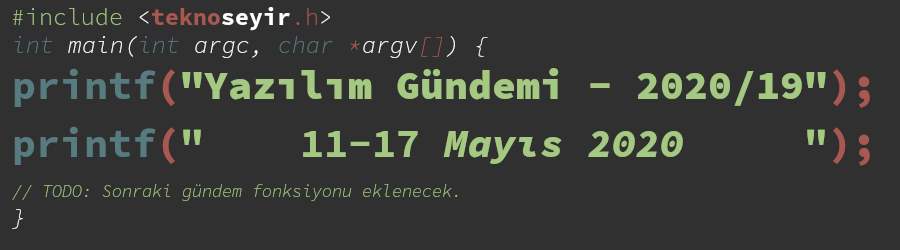
\includegraphics[width=.9\linewidth]{gorseller/yazilim-gundemi-banner.png}
\end{center}

\begin{center}
\href{../18/yazilim-gundemi-2020-18.pdf}{< Önceki Gündem} | \textbf{11-17 Mayıs 2020} | \href{../20/yazilim-gundemi-2020-20.pdf}{Sonraki Gündem >}

\href{https://teknoseyir.com/blog/yazilim-gundemi-2020-19}{TeknoSeyir'de Oku}
\end{center}

\section{Yanlış ayarlanmış Firebase veritabanları binlerce Android uygulamasının \href{https://www.theregister.co.uk/2020/05/12/report\_thousands\_of\_android\_apps/}{kullanıcı verilerinin sızmasına yol açtı}}
\label{sec:orgf9e21d7}
Firebase, genelde mobil ve front-end geliştiricileri için içerisinde
veritabanından, uygulama içi mesajlaşmaya kadar birçok ürünü barındıran bir
Google hizmeti. Gündeme girmesine neden olan ise sunduğu veritabanı
ürünlerinin yanlış konfigüre edilmesinden doğan bazı güvenlik sorunları.
Comparitech isimli firma geçtiğimiz haftanın başında \href{https://www.comparitech.com/blog/information-security/firebase-misconfiguration-report/}{blog sitesinde
yayınladığı yazı} ile bazı Android uygulamalarının kaynak kodlarını açarak,
içerisinden Firebase veritabanı URL'lerini alıp kullanıcı verilerine
erişebildiklerini açıkladılar.

\begin{figure}[htbp]
\centering
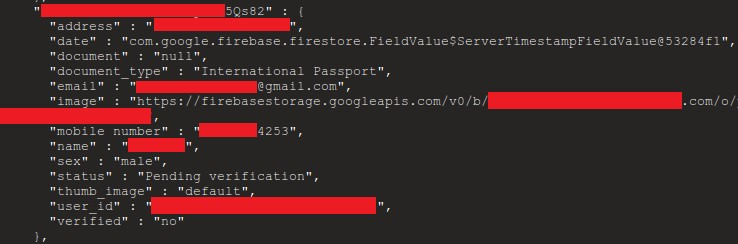
\includegraphics[width=.9\linewidth]{gorseller/firebase-1.jpg}
\caption{Sızan bilgiler arasında binlerce E-posta adresi, telefon numarası, parola, ad soyad ve hatta GPS verisi bile mevcut.}
\end{figure}

Comparitech Güvenlik Araştırması Takım Lideri Bob Diachecko'nun açıkladığına
göre 515.735 Android uygulaması incelenmiş ve bunların içerisinden 4.282
uygulamanın hassas kullanıcı verilerini sızdırığını tespit etmiş.

Firmanın bu güvenlik açığını ortaya çıkarmak için kullandığı ise çok basit
hiçbir yüksek teknoloji ürünü gerektirmeyen bir yöntem. Şöyle ki; uygulamanın
kaynak kodları (biliyorsunuz ki APK dosyaları aslında kaynak kodların bir
çeşit sıkıştırılmış hali ve gerekli uygulamalar ile açılabiliyorlar)
içerisinde "*.firebaseio.com" ifadesini aramak ve buldukları tüm bağlantıların
sonuna ".json" ekleyerek istek göndermek. Eğer ilgili veritabanı yanlış
ayarlanmışsa bu isteğin cevabı tüm veritabanının içeriğinin JSON formatında
sunulmuş hali oluyor. Burada hatırlatmak lazım ki, APK dosyanız şifrelenmiş
(encrypted) olsa bile veritabanınızın URL'sini bir string değişkeninde
tuttuğunuz için yine görülebiliyor.

Comparitech firması 22 Nisan tarihinde bu güvenlik sorununu Google'a bildirmiş
ve Google'da "biz geliştiricilere yanlış konfigüre edilmiş durumlar için
bildirim gönderiyoruz. Bu durum için de etkilenen uygulamaların
geliştiricilerini bilgilendireceğiz" demiş. Eğer sizin de Firebase veritabanı
ürünlerini kullanan bir uygulamanız varsa açığın olup olmadığını kontrol
ederek ve \href{https://firebase.google.com/docs/database/security}{ilgili dokümantasyon sayfalarını} detaylıca inceleyerek olası bir
güvenlik sızıntısının önüne geçebilirsiniz. Hassas verileri veritabanında
şifrelenmiş bir şekilde tutmanın ne kadar önemli olduğunu bir kez daha anlamış
olduk.
\section{Deno \href{https://deno.land/v1}{1.0 yayınlandı}}
\label{sec:orged90bc7}
Gün geçmiyor ki yeni bir JavaScript teknolojisi daha çıkmasın. Şaka bir yana,
bu yeni teknoloji diğerlerine göre daha fazla gündemde kaldı ve konuşuldu.
Node.js'e alternatif olarak geliştirilen(fork değil), yine Node.js'i yaratan
kişinin de (Ryan Dahl) yazarları arasında olduğu \href{https://deno.land/}{Deno} projesinin ilk stabil
versiyonu 1.0, geçtiğimiz hafta içerisinde duyuruldu. Deno da Node.js gibi
sunucu tarafında JavaScript çalıştırmaya yarayan bir runtime çözümü.

Deno'nun neden ortaya çıktığını anlamak için önce Node.js'in sorunlarını
anlamak gerekiyor. Node.js'de \texttt{Promise} yapısının olmaması, güvensiz bir
runtime'a sahip olması, paket yönetimi, testler vb. konularda içerisinde bir
çözüm barındırmaması gibi sorunlar uzun zamandır Node.js kullananlar
tarafından dile getiriliyordu fakat bu ihtiyaçlar hep üçüncü parti araçlar
tarafından giderilebiliyordu. Node.js paket yönetimi için \texttt{npm} ile birlikte
geliyor fakat \texttt{npm} doğrudan Node.js tarafından geliştirilen bir araç değil,
kontrol onlarda değil yani. Güvensiz runtime'dan kast edilen ise Node.js'in
kontrolsüz sistem çağrıları (sys calls) yapabiliyor olması. Node.js ile bir
JavaScript dosyası çalıştırdığınızda o işlem, sistemin tüm kaynaklarını
kullanabiliyordu. Örneğin istediği bir dosyayı okuyabilir ya da yazabiliyordu.
Bunun gibi Node.js'in tasarımından kaynaklanan diğer sorunlar için doğrudan
Node.js'in yaratıcılarından Ryan Dahl'ın JSConf EU 2018 etkinliğinde yaptığı
konuşmayı \href{https://www.youtube.com/watch?v=M3BM9TB-8yA}{buraya tıklayarak izleyebilirsiniz}.

\begin{figure}[htbp]
\centering

\includegraphics[height=4cm]{gorseller/deno-logo.png}
\caption{Deno'nun resmî logosu}
\end{figure}

Gel gelelim Deno'ya\ldots{} Deno'da yukarıdaki birçok sorun çözülmüş durumda, artık
tek bir araç kurarak geliştirme ortamınızdaki birçok ihtiyacınızı
giderebiliyorsunuz. Şöyle ki:
\begin{itemize}
\item \texttt{deno run}: Bu komut ile kodlarınızı direkt çalıştırabilirsiniz. Üstelik
kendi içerisinde TypeScript desteği ile geliyor, yani TypeScript
kodlarınızı derleyici ile JavaScript'e dönüştürüp o şekilde kullanmanıza
gerek yok. Direkt \texttt{deno run deneme.ts} şeklinde çalıştırabiliyorsunuz.
\item \texttt{deno bundle}: Bu komuta parametre olarak verdiğiniz bir kaynak kod dosyası
(JS ya da TS olabilir), tüm bağımlılıklarıyla birlikte tek bir dosya haline
getiriliyor. bir dosya haline getirmeye yarıyor.
\item \texttt{deno fmt}: Kodlarınızın otomatik olarak formatlanmasını sağlar.
\item \texttt{deno doc}: Bir modül için tanımlanmış dokümantasyon metinlerini
gösteriyor.
\item \texttt{deno test}: Projeniz için yazdığınız testleri bu komut yardımıyla
çalıştırabiliyorsunuz.
\end{itemize}

\begin{figure}[htbp]
\centering
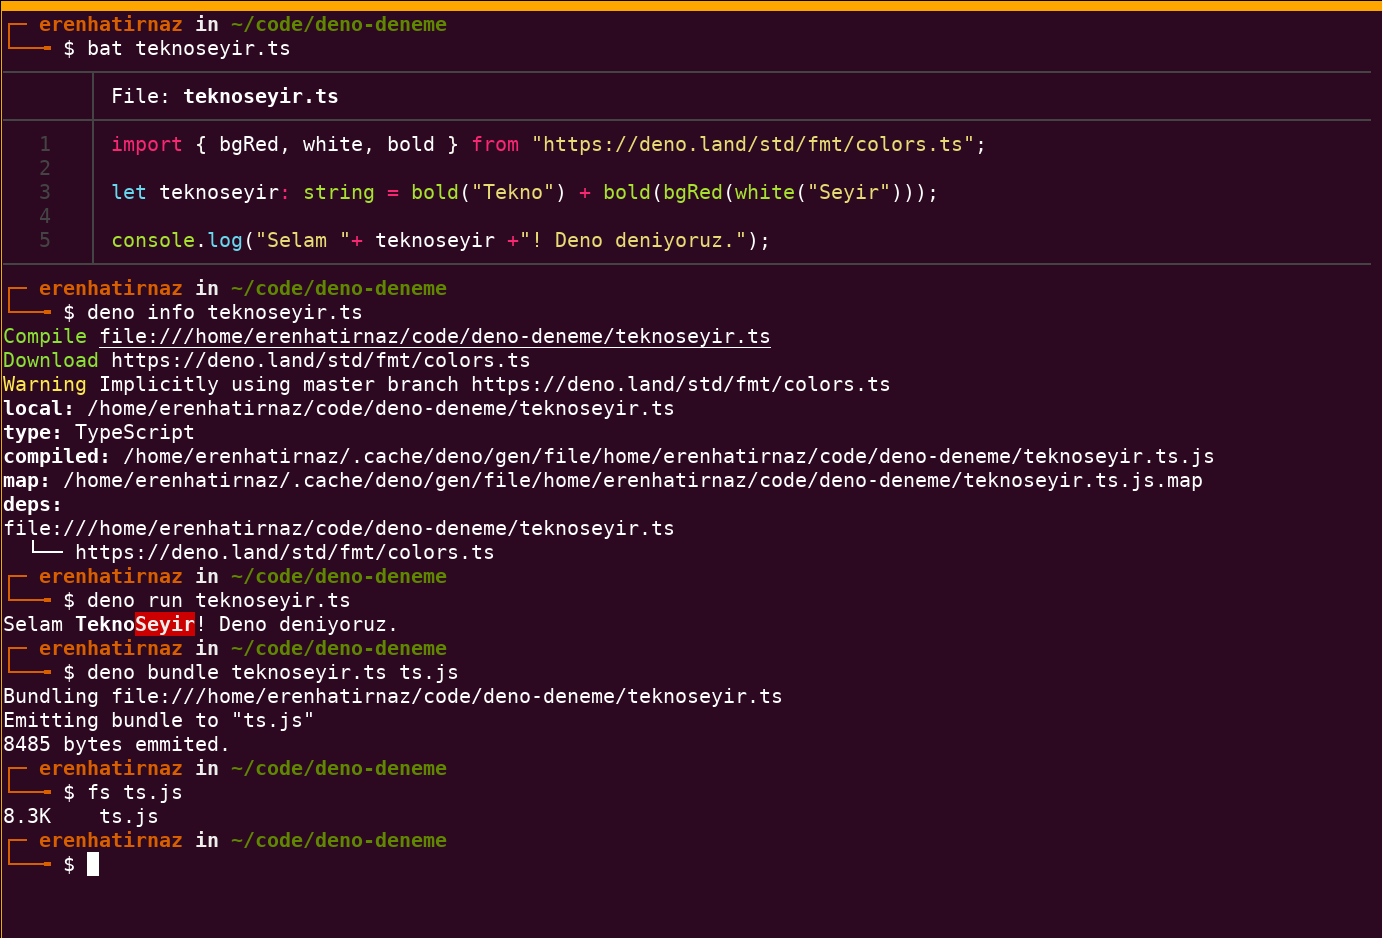
\includegraphics[width=.9\linewidth]{gorseller/deno-deniyoruz.png}
\caption{Deno'yu sizler için denedim. Örnek tabii ki çok basit ama Node.js'e göre daha hızlı geliştirebildim.}
\end{figure}

Yukarıdaki örnekte de gördüğünüz gibi hiç package.json dosyası gibi şeylerle
uğraşmadan doğrudan ilgili dosyanın adresini import olarak belirterek dosyama
ekledim ve \texttt{deno info} komutuyla hem kodlarımı derledim hem de bağımlılıkları
indirdim. \texttt{deno info} komutunu çalıştırmak zorunda değilsiniz elbette direkt
\texttt{deno run teknoseyir.ts} komutu da çalıştırabilirsiniz. Eğer siz de yukarıdaki
dosyayı denemek isterseniz bu adresten indirip, deneyebilirsiniz:
\url{https://gist.github.com/erenhatirnaz/fc6e726fff2731bc1ed763bb2ba7d3e8}

Hepimizin aklındaki soru ise "Node.js'yi bitirir mi?" olduğunu tahmin ediyorum
fakat henüz böyle bir çıkarım yapabilmek için çok erken olsa da sunduğu
özellikler bakımından gerçekten umut vaat ettiğini düşünüyorum. Node.js için
yazılmış kütüphaneler için henüz bir uyumluluk çözümü yok fakat şu an
geliştirilme aşamasındaymış, ileride Node.js için de yazılmış kütüphaneleri
kullanabilir hale geldiğimizde belki o zaman Node.js'in ömrünü konuşmaya
başlayabiliriz. Bakalım JavaScript ekosistemini ileride ne gibi değişlikler
bekliyor. Hep birlikte göreceğiz.

Deno hakkında daha detaylı bilgiler için konu başlığına eklediğim bağlantıya
tıklayabilir ya da DevNot sitesinden Zafer Ayan'ın yazdığı \href{http://devnot.com/2020/deno-nedir-nodejsin-sonunu-getirir-mi/}{şu türkçe yazıyı
okuyabilirsiniz}.

Siz Deno hakkında ne düşünüyorsunuz? Deneyebildiniz mi? Denediyseniz
olumlu/olumsuz eleştirileriniz neler? Yorumlar bölümünde fikir alışverişi
yapalım.
\section{Unreal Engine 5 \href{https://www.unrealengine.com/en-US/blog/a-first-look-at-unreal-engine-5}{ilk bakış duyuruldu}}
\label{sec:org4003b1a}
Geçtiğimiz hafta içerisinde Epic Games firmasının sahip olduğu Unreal Engine
oyun motorunun 5 numaralı versiyonunun ilk bakış videoları ve yayınlanma
süreci hakkında bazı detaylar duyuruldu. Zaten geçtiğimiz haftanın olay
yaratan konularından biri de bu oldu.

\begin{itemize}
\item \href{https://www.youtube.com/watch?v=qC5KtatMcUw}{Konuyla ilgili YouTube videosu}
\end{itemize}

Front-end geliştirme alanından bile daha uzak olduğun oyun geliştirme alanıyla
ilgili bir haber olduğu için teknik kısımlarını pek iyi yorumlayamayacağım
fakat duyurulan şeyleri anladığım ölçüde sizlere aktarmaya çalışayım:

\begin{itemize}
\item \textbf{Nanite}: Bu yeni teknoloji sayesinde artık 3D tasarım yapan sanatçılar
poligon sayısını çok kafasına takmadan hayallerindeki tasarımları dijital
ortama aktarabilecekler. ZBrush ile taratılmış nesnelerden, CAD verilerine
kadar birçok obje bu şekilde kullanılabilecek. Gerçek zamanlı olarak
çalışan bu teknoloji kalite kaybı olmadan daha hızlı geliştirme yapmaya
olanak sağlayacak.
\item \textbf{Lumen}: Bu sürümle birlikte gelecek olan tamamen dinamik aydınlatma
çözümü. Bu özelliği okuyunca benim aklıma NVIDIA'nin RTX çözümü geldi. Bu
da aynı onun gibi ışığın dinamik olarak hesaplanmasını ve dolayısıyla
ortamlara ve zamana göre nesnelere vuran ışığın değişmesini sağlıyor. Tabii
ki bu da gerçek zamanlı olarak GPU üzerinde hesaplanıyor ve oyuna
yansıtılıyor. Teknik bilgim olmadığı için bu özelliğin RTX ile bağlantılı
olup olmadığını bilemiyorum fakat konu hakkında bilgisi olan arkadaşlar
yorumlar bölümünde belirtirse buraya ekleme yapabilirim.
\end{itemize}

Unreal Engine 5 ile birlikte çekirdeğe eklenen yeni teknolojiler bu
şekildeydi. Unreal Engine 5 ön izleme sürümünün 2021'in ilk ayları içerisinde
duyurulması beklenirken, tamamen stabil sürümün ise 2021'in daha ileri
tarihlerinde yayınlanması planlanıyor. Unreal Engine 4 kullanan
geliştiricilerin 5'e geçebilmeleri için uyumluluk çalışmalarının da devam
ettiğini, geçiş sürecini kolaylaştırmak için çaba gösterdiklerini
aktarıyorlar.

Unreal Engine 5 ile birlikte Epic Games bir de \href{https://www.unrealengine.com/en-US/blog/epic-online-services-featuring-epic-account-and-game-services}{yeni bir servis duyurdu}: \href{https://dev.epicgames.com/en-US/services}{Epic
Online Services}. Bu yeni servis sayesinde oyun geliştiricileri oyunlarına daha
kolay bir şekilde çoklu oyuncu desteği eklemenin yanı sıra, lider tabloları,
başarımlar vb. şeyleri de ekleyebilecekler. Üstelik bu hizmet tüm
geliştiriciler için ücretsiz olarak sunuluyor. Epic Games, bu hizmeti sadece
kendi oyun mağazası için sınırlamamış platformlar arası (cross-platform)
desteği de eklemiş. Yani Playstation'dan XBox'a oradan iOS ve Android'e kadar
birçok platformda oyuncular aynı şeylere sahip olabilecek.

Son olarak ise artık Unreal Engine kullanan geliştiriciler ve oyun yapımcıları
yıllık gelirleri 1 milyon dolar olana kadar Unreal Engine'e lisans ücreti
ödemek zorunda değiller. Lisanslama ile ilgili sorular için \href{https://www.unrealengine.com/faq}{şu bağlantıda yer
alan sıkça sorulan sorular} kısmına göz atabilirsiniz.

Bu gelişme oyun geliştirme dinamiklerini nasıl etkiler, ilerleyen süreçlerde
bizi neler bekliyor pek bilemiyorum ama oyun geliştirme alanında çalıştığını
tahmin ettiğim Sosyal'den @ardazeytin arkadaşımızın yazdığı şu gönderiye
bakabilirsiniz: \url{https://teknoseyir.com/durum/1265228}.

Oyun geliştirme alanında çalışan başka arkadaşlar varsa bu konu hakkında
düşündüklerini yorumlar bölümünde dile getirirse çok memnun olurum.
\section{Eclipse Foundation \href{https://newsroom.eclipse.org/news/announcements/open-source-software-leader-eclipse-foundation-announces-transition-europe-part}{Avrupa'ya taşınıyor}}
\label{sec:orgd576c30}
\begin{center}

\includegraphics[height=3cm]{gorseller/eclipse-foundation-tasindik.jpg}
\end{center}

Çoğunlukla Java IDE'si olarak tanıdığımız Eclipse, aslında \href{https://www.eclipse.org/}{Eclipse Foundation}
isimli bir yapının parçası. Geçtiğimiz hafta içerisinde ise Eclipse
Foundation, tüzel kişiliklerini Brüksel'e taşıyarak bir Uluslararası kâr amacı
gütmeyen dernek haline geleceklerini açıkladılar.

Şu anda Amerika merkezli bir vakıf olan Eclipse Foundation, taşınma nedeniyle
ilgili açıklamalarda genelde "üyelerimiz ve katkı sağlayanlarımızın çoğu
Avrupa'da olduğu için biz de onlara yakın olmak için merkezimizi oraya
taşıyoruz" şeklinde özetliyorlar fakat ben Amerika'daki güncel siyasi durumun
da konu üzerinde etkisi olabileceğini düşünüyorum. Bir de tüzel kişilikle
ilgili bazı yasal kolaylıklardan bahsedilmiş sanırım fakat alanım olmayan bir
konu olduğu için pek fazla bir şey anlamadım.

Taşınma süreciyle ilgili detaylar şu şekilde özetlenebilir:
\begin{itemize}
\item Uluslararası kar amacı gütmeyen derneğin resmî işlemlerinin Temmuz 2020'de
tamamlanması bekleniyor.
\item Fiziksel olarak Avrupa'da barındırılan, üzerinde GitLab kurulu sunucularda
tüm projelerinin kaynak kodlarına ve dokümanlarına bu yılın yaz ayları
itibariyle erişilebilecek. Burası geliştiriciler ve katkı sağlayanlar için
üçüncü bir seçenek olarak sunulacak.
\item Eclipse ve Eclipse Foundation isimleri ve markaları yeni Belçika varlığı olarak
kontrol edilecek.
\item Eclipse Foundation zaten hali hazırda Kanada ve Avrupa (Almanya ofisi
mevcuttu) üzerinde eş zamanlı yönetildiği için vakfın operasyonlarının en
düşük seviyede etkileneceği tahmin ediliyor.
\end{itemize}

Biz geliştiricileri pek fazla etkileyeceğini sanmıyorum ama yinede
sektörümüzdeki önemli bir vakıfın böyle büyük bir taşınma işine girişmesini
gündeme almak istedim. Daha detaylı bilgiler için konu başlığına eklediğim
bağlantıya tıklayabilir ya da \href{https://www.eclipse.org/europe/faq.php}{şu adresdeki sıkça sorulan sorular sayfası}nı
ziyaret edebilirsiniz. Eclipse Foundation Europe ana sayfası için burayı
ziyaret edebilirsiniz: \url{https://www.eclipse.org/europe/}
\section{Firefox 77 ile birlikte \texttt{<input>} ve \texttt{<textarea>} elemanlarında \href{https://www.fxsitecompat.dev/en-CA/docs/2020/text-exceeding-maxlength-will-no-longer-be-truncated-when-pasted-into-input-or-textarea/}{davranış değişiklikleri geliyor}}
\label{sec:org4d6b3a0}
Mozilla tarafından geliştirilen web tarayıcısı Firefox'un bir sonraki sürümü
olarak yayınlanacak 77 numaralı sürümünde \texttt{<input>} ve \texttt{<textarea>}
elemanlarında değişiklikler olacağı geçtiğimi hafta Firefox Site Compatibility
sitesinde duyuruldu.

Artık bu elemanlara kopyala/yapıştır ile bir içerik yapıştırdığımızda eğer
içeriğin boyutu, elemanın \texttt{maxlength} property'sindeki boyuttan büyükse,
yapıştırdığımız içerik otomatik olarak kırpılmayacak. Yani kullanıcılar o
elemana daha uzun içerikler yapıştırabilecekler fakat bu demek değil ki
Firefox bizim koyduğumuz kuralı görmezden geliyor. Firefox, \texttt{maxlength}
değerine uymayan formları submit etmemeye devam edecek. Yapılan davranış
değişikliğinin sebebi ise kullanıcıların şifre yönetim uygulamalarının ilgili
elemana otomatik olarak yapıştırdığı şifrelerin kırpılmamasını sağlamak. Yani
kullanıcının "acaba parolamla ilgili bir sıkıntı mı var" endişesini gidermeye
yönelik. Eğer girilen metin olması gerekenden uzunsa Firefox kullanıcıya şöyle
bir mesaj gösterecekmiş: "Lütfen bu metini 20 karakter ya da daha az olacak
şekilde kısatın (şu an 30 karakter kullanıyorsunuz)".

Çalışan projelerimizi doğrudan etkileyecek bir durum göremiyorum ama yine de
dikkate almaya değer bir davranış değişikliği olduğu için değinmeden geçmek
istemedim. Daha detaylı bilgiler ve referanslar için konu başlığına eklediğim
bağlantıya tıklayabilirsiniz.
\section{\href{https://github.blog/changelog/2020-05-11-github-cli-allows-you-to-close-reopen-and-add-metadata-to-issues-and-pull-requests/}{GitHub Desktop 2.5} ve \href{https://github.blog/changelog/2020-05-11-github-cli-allows-you-to-close-reopen-and-add-metadata-to-issues-and-pull-requests/}{GitHub CLI 0.8} sürümü yayınlandı}
\label{sec:org6e09198}
GitHub'ın grafiksel masaüstü uygulaması ve komut satırı üzerinden çalışan
aracı geçtiğimiz hafta içerisinde yeni sürümlerine kavuşturlar. Yeni sürümler
ile gelen bazı özellikler şu şekilde:
\subsection{[GitHub Desktop] Etiket oluşturma ve gönderme}
\label{sec:org9115f30}
\url{gorseller/github-desktop-tag.gif}

Artık GitHub uygulaması üzerinden yeni git etiketleri (\texttt{git tag}) oluşturup,
bunları GitHub.com üzerindeki uzak deponuza gönderebileceksiniz. Tabii ki
var olan etiketleri de listeleme özelliği mevcut.
\subsection{[GitHub CLI] Isseu ve Pull Requestleri kontrol etme}
\label{sec:orgf37feeb}
GitHub CLI üzerinden zaten bir proje üzerinde issue oluşturabiliyor ya da
pull request gönderebiliyorduk fakat işlemler sadece bunlarla kısıtlıydı.
Diğer ek işlemler için tarayıcıda açmak gerekiyordu. Bu sürümle birlikte
artık issue ve pull requestlerimizi yaratırken onlara label, reviewer,
projects, milestone gibi ek bilgiler iliştirebileceğiz. Aynı zamanda \texttt{gh pr
	 close}, \texttt{gh pr reopen} ve \texttt{gh issue close}, \texttt{gh issue reopen} gibi komutlarla
ilgili issue ya da pull requestleri açıp kapatabileceğiz. Komut satırı
kullanmayı seven biri olan beni mutlu eden gelişmeler fakat henüz tam zamanlı
kullanılabilecek kadar gelişmedi hele bir 1.0 sürümü çıksın bakalım\ldots{}
\section{SourceHut, PeerTube projesini desteklemek için \href{https://sourcehut.org/blog/2020-05-15-peertube-bootstrap-fund/}{fon programını duyurdu}}
\label{sec:org7775b05}
\href{https://sourcehut.org/}{SourceHut}'ın ne olduğundan ve felsefesinden önceki yazılım gündemi yazılarının
birinde (bkz: \href{../../2019/17/yazilim-gundemi-2020-17.pdf}{Yazılım Gündemi - 2020/17}) bahsetmiştim. O yazıyı okumayanlar
için kısa bir özet: SourceHut da GitHub ve GitLab gibi uzak bir git deposu
hizmeti fakat tamamen özgür yazılım prensiplerine göre ve açık kaynak şekilde
geliştiriliyor (ve JavaScript kullanmıyor). \href{https://joinpeertube.org/}{PeerTube} ise YouTube'a benzer,
gelişmiş ve dağıtık bir video paylaşma platformu. Teknik detaylarına pek fazla
hakim değilim fakat siz bir PeerTube sitesine bir video yüklediğinizde aslında
bir çeşit torrent paylaşmış gibi oluyorsunuz ve tarayıcı üzerinden o videoyu
izleyen diğer kişiler de hem indiriyor hem de diğer kullanıcılar için
gönderiyor. Bu sayede dağıtık bir yapı kurulmuş oluyor. İsterseniz sizde kendi
sunucularınızda bir PeerTube ayağa kaldırabilir ve bu ağın bir parçası
olabilirsiniz. İkisi de çok sevdiğim ve bir çeşit gönül bağı kurduğum
projeler. Hazır yeri gelmişken ikisini birden gündemde konuk etmek istedim :).

SourceHut ise geçtiğimiz hafta içerisinde PeerTube projesini desteklemek ve
içerik sayısını arttırmak için bir çeşit fon ayırdığını açıkladı. 5.000\$'lık
bu fon sayesinde PeerTube'a içerik üretmek isteyen kişilere ekipman desteği ve
kitle fonlama araçları sağlanacak. Kitle fonlama aracı ise yine özgür yazılım
prensipleriyle geliştirilen \href{https://liberapay.com/}{Librepay}. Fakat bu fondan faydalanabilmenin bazı
şartları var:
\begin{itemize}
\item Hali hazırda başka bir platform üzerinde videolu içerik üretmiyor olmanız
gerekiyor fakat bu o kadar sert bir kural değil sanırım, birkaç video
üretmişseniz yine de başvurunuzda bunu açıkca belirterek değerlendirilme
süreçlerine dahil olabiliyorsunuz.
\item Videolarınızı \textbf{sadece PeerTube'a} yükleyebilirsiniz. YouTube, Vimeo vb.
platformlarda PeerTube için özel ürettiğiniz içerikler bulunamaz.
\item Oluşturduğunuz video içerikler \href{https://creativecommons.org/}{Creative Commons} lisansları ile
paylaşılmalıdır.
\item En az 5 video üretmeniz bekleniyor. Eğer bu 5 videodan sonra videolu içerik
üretmenin size göre olmadığına karar verirseniz fon yardımıyla aldığınız
ekipmanları geri vermeniz gerekiyor.
\item Librepay üzerinden aylık en az \$20'dan fazla kazanmaya başladığınızda,
devam eden barındırma maliyetleri tüm içerik oluşturucular arasında eşit
olarak paylaştırılacak. Yani şimdilik aylık \$45 olan bu maliyet içerik
oluşturucular arasında eşit bir şekilde bölüştürülür. Librepay gelirinizin
\%25'inden fazla ödeme yapmanız asla beklenmiyor; SourceHut gerisini
tamamlıyor.
\end{itemize}

Eğer bu fona başvurmak isterseniz sir@cmpwn.com e-posta adresine, başlığı
"\emph{PeerTube bootstrap application: <ad soyad>}" olan ve içeriğinde de kendinizi
tanıtarak ne tür bir içerik oluşturmak istediğinizden bahsedebilirsiniz.

SourceHut'ın kendi barındırdığı PeerTube hizmeti için burayı ziyaret
edebilirsiniz: \href{https://spacepub.space/}{SpacePub}. Diğer detaylar için konu başlığına eklediğim
bağlantıya tıklayabilirsiniz.

Geçtiğimiz hafta SourceHut'daki diğer bazı gelişmeler de bu şekilde:
\begin{itemize}
\item Mayıs 2020 için SourceHut'da pişen özellikler \href{https://sourcehut.org/blog/2020-05-15-whats-cooking-may-2020/}{yazısı yayınlandı}.
\item SourceHut'a \href{https://sourcehut.org/blog/2020-05-11-sourcehut-plus-plan-9/}{Plan 9 desteği eklendi}.
\end{itemize}
\section{Yaklaşan Online Etkinlikler \#EvdeKal}
\label{sec:org3f9c437}
\begin{longtable}{|p{9.5cm}|l|}
\hline
Etkinlik İsmi & Tarihi\\
\hline
\endfirsthead
\multicolumn{2}{l}{Önceki sayfadan devam ediyor} \\
\hline

Etkinlik İsmi & Tarihi \\

\hline
\endhead
\hline\multicolumn{2}{r}{Devamı sonraki sayfada} \\
\endfoot
\endlastfoot
\hline
\href{https://kommunity.com/bilge-adam-teknoloji/events/react-ile-javascript-uygulamalari-gelistirme-b70b2cb9}{React ile JavaScript Uygulamaları Geliştirme} & 18 Mayıs 16:00\\
\href{https://kommunity.com/cloud-and-serverless-turkey/events/ramazan-ozel-8-bulutta-yuksek-performansli-ve-verimli-sistem-tasarlama-a72398fb}{Bulutta Yüksek Performanslı ve Verimli Sistem} & 18 Mayıs 23:00\\
\href{https://kommunity.com/pgtr/events/postgresql-sohbetleri-18-postgresqlde-gozlemleme-monitoring-d78fab87}{PostgreSQL Sohbetleri 18: PostgreSQL'de gözlemleme} & 19 Mayıs 13:30\\
\href{https://kommunity.com/tracikkaynak/events/acik-seminer-22-gun-postgresql-53dbbb44}{Açık Seminer 22. Gün: PostgreSQL'e Giriş} & 19 Mayıs 13:00\\
\href{https://kommunity.com/bilge-adam-teknoloji/events/net-core-refit-kullanimi-f9c2215b}{.NET Core Refit Kullanımı} & 19 Mayıs 14:00\\
\href{https://kommunity.com/jstanbul/events/deno-yeni-javascript-runtimei-3bc240d7}{Deno: Yeni JavaScript Runtime'ı} & 19 Mayıs 21:15\\
\href{https://kommunity.com/teknopark-istanbul-yazilimci-bulusmalari/events/orneklerle-unit-testing-ve-tdd-3f5cc824}{Örneklerle Unit Testing ve TDD} & 20 Mayıs 12:30\\
\href{https://kommunity.com/tracikkaynak/events/acik-seminer-23-gun-postgressql-temel-bilgiler-b31504bc}{Açık Seminer 23. Gün: PostgreSQL Temel Bilgiler} & 20 Mayıs 14:00\\
\href{https://kommunity.com/bilge-adam-teknoloji/events/html-ve-css-ile-web-arayuz-tasarimi-48e9156f}{HTML ve CSS ile Web Arayüz Tasarımı} & 20 Mayıs 18:00\\
\href{https://kommunity.com/bilge-adam-teknoloji/events/building-net-core-31-serverless-application-in-aws-5c948e36}{Building .NET Core 3.1 Serverless Application in AWS} & 20 Mayıs 22:00\\
\href{https://kommunity.com/tracikkaynak/events/acik-seminer-24-gun-postgresde-kurulus-ve-gelisim-yolculugu-80e1191a}{Açık Seminer 24. Gün: Postgres’de Kuruluş ve Gelişim Yolculuğu} & 21 Mayıs 14:00\\
\href{https://kommunity.com/frontend-istanbul/events/asynchronous-code-execution-under-the-hood-605ea817}{Asynchronous Code Execution Under the Hood} & 21 Mayıs 18:00\\
\href{https://kommunity.com/cloud-and-serverless-turkey/events/ramazan-ozel-9-aws-cloud-ogrenmeye-nereden-ve-nasil-baslarim-7d516704}{AWS - Cloud öğrenmeye nereden ve nasıl başlarım?} & 21 Mayıs 23:00\\
\href{https://kommunity.com/mdisec-cyber-security-twitch-streams/events/hackerconfstream-virtual-cyber-security-conference-b7bd6be7}{HackerConf.Stream Virtual Cyber Security Conference} & 22 Mayıs 09:59\\
\href{https://kommunity.com/tracikkaynak/events/acik-seminer-25-gun-gelistiriciler-icin-postgresql-e7c76ef0}{Açık Seminer 25. Gün: Geliştiriciler için PostgreSQL} & 22 Mayıs 14:00\\
\href{https://kommunity.com/mavidurakio/events/s1e43-unity-ile-oyun-programlamaya-giris-101-23658c44}{Unity ile Oyun Programlamaya Giriş 101} & 22 Mayıs 21:15\\
\hline
\end{longtable}
\section{Diğer Haberler}
\label{sec:orgd165855}
\begin{itemize}
\item GitLab.com 13.0 sürümüne \href{https://about.gitlab.com/releases/2020/05/06/gitlab-com-13-0-breaking-changes/}{güncellenecek}. 22 Mayıs günü kesintiler
yaşanabilir.
\item GitHub "Organizastion secrets" \href{https://github.blog/changelog/2020-05-14-organization-secrets/}{özelliğini duyurdu}.
\item Java \href{https://blogs.oracle.com/java/our-world-moved-by-java}{25 yaşında}.
\item Rust \href{https://blog.rust-lang.org/2020/05/15/five-years-of-rust.html}{5 yaşında}.
\item Amazon ve Red Hat yeni \href{https://www.zdnet.com/article/amazon-red-hat-openshift-announced-for-public-cloud-kubernetes-users/}{ortak projelerini duyurdu}: \href{https://aws.amazon.com/quickstart/architecture/openshift/}{Amazon Red Hat OpenShift}.
\href{https://www.redhat.com/en/blog/red-hat-and-aws-extend-collaboration-introducing-amazon-red-hat-openshift}{Alternatif}
\item AWS, Kubernetes için bulut geliştirme kitini \href{https://siliconangle.com/2020/05/13/aws-open-sources-cdk8s-make-kubernetes-easier-use/}{açık kaynak hale getirdi}:
\href{https://siliconangle.com/2020/05/13/aws-open-sources-cdk8s-make-kubernetes-easier-use/}{cdk8s}.
\item AWS kendi ARM-tabanlı çipi için \href{https://aws.amazon.com/blogs/aws/new-m6g-ec2-instances-powered-by-arm-based-aws-graviton2/}{yeni EC2 servisini tanıttı}: EC2 M6g.
\item Google Cloud VMware Engine \href{https://cloud.google.com/blog/topics/hybrid-cloud/announcing-google-cloud-vmware-engine}{Genel Erişilebilir (GA) hale geldi}.
\item Amazon Kendra \href{https://techcrunch.com/2020/05/11/amazon-releases-kendra-to-solve-enterprise-search-with-ai-and-machine-learning/}{Genel Erişilebilir (GA) hale geldi}.
\item JetBrains'den haberler:
\begin{itemize}
\item YouTrack, 10 kişilik takımlar \href{https://blog.jetbrains.com/youtrack/2020/05/youtrack-is-now-free-for-10/}{için ücretsiz oldu}.
\item Python Geliştiricileri Anketi 2019 \href{https://www.jetbrains.com/lp/python-developers-survey-2019}{sonuçları açıklandı}.
\item MPS 2020.1 \href{https://blog.jetbrains.com/mps/2020/05/mps-2020-1-has-been-released/}{sürümü yayınlandı}.
\item IntelliJ IDEA, Çince, Japonca ve Korece dil desteği için \href{https://blog.jetbrains.com/idea/2020/05/intellij-idea-localization-eap1/}{erken erişim
programı başlatıldı}.
\end{itemize}
\item TypeScript programlama dilinin \href{https://devblogs.microsoft.com/typescript/announcing-typescript-3-9/}{3.9 sürümü duyuruldu}.
\item Erlang/OTP \href{https://www.erlang.org/news/140}{23 sürümü yayınlandı}.
\item Switft 5.3 ile birlikte Windows ve bazı Linux dağıtımları \href{https://www.infoq.com/news/2020/05/swift-5-3-windows-linux/}{için destek
gelecek}.
\item WebAssembly çalıştırabilen ilk \href{https://medium.com/wasmer/announcing-the-first-java-library-to-run-webassembly-wasmer-jni-89e319d2ac7c}{Java kütüphanesi duyuruldu}: \href{https://github.com/wasmerio/java-ext-wasm}{Wasmer JNI}.
\item Next.js \href{https://nextjs.org/blog/next-9-4}{9.4 sürümü yayınlandı}.
\item Bootstrap \href{https://blog.getbootstrap.com/2020/05/12/bootstrap-4-5-0/}{4.5.0 sürümü yayınlandı}.
\item Apache Kafka, Apache ZooKeeper \href{https://www.confluent.io/blog/removing-zookeeper-dependency-in-kafka/}{bağımlığımından kurtuluyor}.
\item PostgreSQL 12.3, 11.8, 10.13, 9.6.18 ve 9.5.22 \href{https://www.postgresql.org/about/news/2038/}{sürümleri yayınlandı}.
\item CockroachDB \href{https://www.cockroachlabs.com/blog/cockroachdb-20-1-release/}{20.1 sürümü duyuruldu}.
\item MongoDB \href{https://www.mongodb.com/blog/post/introducing-mongodb-for-vs-code}{4.2.6 sürümü yayınlandı}.
\item VSCode için MongoDB eklentisi \href{https://www.mongodb.com/blog/post/introducing-mongodb-for-vs-code}{ön izleme olarak yayınlandı}.
\item HAProxy Data Plane API \href{https://www.haproxy.com/blog/announcing-haproxy-dataplane-api-20/}{2.0 sürümü duyuruldu}.
\item Haxe \href{https://haxe.org/blog/haxe-4.1.0-release/}{4.1.0 sürümü yayınlandı}.
\item Proxmox VE \href{https://www.proxmox.com/en/news/press-releases/proxmox-ve-6-2}{6.2 sürümü yayınlandı}.
\item Zabbix \href{https://www.zabbix.com/rn/rn5.0.0}{5.0.0 sürümü yayınlandı}.
\item Hyperdrive \href{https://blog.hypercore-protocol.org/posts/announcing-hyperdrive-10/}{v10 sürümü duyuruldu}.
\item Mun \href{https://mun-lang.org/blog/2020/05/16/release-mun-v0-2-0/}{v0.2.0 sürümü yayınlandı}.
\end{itemize}
\section{Lisans}
\label{sec:org1c94e5c}
\begin{center}
\begin{center}

\includegraphics[height=1.5cm]{../../../img/CC_BY-NC-SA_4.0.png}
\end{center}

\href{yazilim-gundemi-2020-19.pdf}{Yazılım Gündemi - 2020/19} yazısı \href{https://erenhatirnaz.github.io}{Eren Hatırnaz} tarafından \href{http://creativecommons.org/licenses/by-nc-sa/4.0/}{Creative Commons
Atıf-GayriTicari-AynıLisanslaPaylaş 4.0 Uluslararası Lisansı} (CC BY-NC-SA 4.0)
ile lisanslanmıştır.
\end{center}
\end{document}
